\documentclass[a4paper, 11pt]{article}

\usepackage{amsmath, amssymb, amsthm}
\usepackage{bm}
\usepackage{tikz}
\usepackage{graphicx}
\usepackage{booktabs}
\usepackage{enumitem}

\usepackage[margin=2.5cm]{geometry}
\usepackage[hidelinks]{hyperref}
\usetikzlibrary{positioning}

\title{week2-3}
\author{Xidai Lin}
\date{}
\begin{document}
\maketitle
\section*{1.37}
Using the definition (1.111) together with the product rule of probability,
prove the result (1.112).
\[
H[x,y]=-\int\int p(x,y)ln(p(x,y))dxdy=\int\int p(x,y)[ln(p(y\mid x))+ln(p(x))]
\]
by (1.111) $H[y\mid x]=-\int\int p(y,x)ln(p(y\mid x))dydx$, we have
\[
H[x,y]=H[y\mid x]+H[x]
\]
\section*{1.34}
Use the calculus of variations to show that the stationary point of the
functional (1.108) is given by (1.108). Then use the constraints (1.105),
(1.106), and (1.107) to eliminate the Lagrange multipliers and hence show
that the maximum entropy solution is given by the Gaussian (1.109).

let $H=-\int_{-\infty}^{\infty}p(x)ln(p(x))dx+\lambda_1(\int_{-\infty}^{\infty}p(x)dx-1)+\lambda_2(\int_{-\infty}^{\infty}xp(x)dx-\mu)+\lambda_3(\int_{-\infty}^{\infty}(x-\mu)^2p(x)dx-\sigma^2)$, we have
\[
\frac{\delta H}{\delta p}=-ln(p)-1+\lambda_1+\lambda_2x+\lambda_3(x-\mu)^2=0
\]
So,\[
p(X)=e^{-1+\lambda_1+\lambda_2x+\lambda_3(x-\mu)^2}
\]
let
\[
p(x)=e^{a(x-b)^2+c}
\]
we have
\[
\int_{-\infty}^{\infty}p(x)dx=1\Rightarrow e^c\sqrt{\frac{\pi}{-a}}=1\Rightarrow c=-\frac{1}{2}ln(-a)-\frac{1}{2}ln(\pi)
\]
\[
\int_{-\infty}^{\infty}xp(x)dx=\mu\Rightarrow b=\mu   
\]
\[
\int_{-\infty}^{\infty}(x-\mu)^2p(x)dx=\sigma^2\Rightarrow -\frac{1}{2a}=\sigma^2\Rightarrow a=-\frac{1}{2\sigma^2}
\]
Thus,
\[
p(x)=\frac{1}{\sqrt{2\pi\sigma^2}}e^{-\frac{(x-\mu)^2}{2\sigma^2}}
\]
i.e. the Gaussian distribution.
\section*{1.39}
Consider two binary variables $x$ and $y$ having the joint distribution given
in Table~1.3.

\begin{center}
\textbf{Table 1.3.} The joint distribution $p(x,y)$.

\medskip
\begin{tabular}{crcc}
\toprule
& & \multicolumn{2}{c}{$y$} \\
\cmidrule(lr){3-4}
& & $0$ & $1$ \\
\midrule
$x$ & $0$ & $1/3$ & $1/3$ \\
    & $1$ & $0$   & $1/3$ \\
\bottomrule
\end{tabular}
\end{center}

Evaluate the following quantities.
\begin{enumerate}[label=(\alph*), nosep]
    \item $H[x]$
    \item $H[y]$
    \item $H[y\mid x]$
    \item $H[x\mid y]$
    \item $H[x,y]$
    \item $I[x,y]$
\end{enumerate}

Draw a diagram to show the relationship between these various quantities.
\subsection*{a}
\[
H[x]=-(\frac{1}{3}ln(\frac{1}{3})+\frac{2}{3}ln(\frac{2}{3}))=\frac{1}{3}ln(\frac{27}{4})
\]
\subsection*{b}
\[
H[y]=\frac{1}{3}ln(\frac{27}{4})
\]
\subsection*{e}
\[
H[x,y]=\frac{1}{3}ln(3)*3=ln{3}
\]
\subsection*{c}
\[
H[y\mid x]=H[x,y]-H[x]=ln(3)-\frac{1}{3}ln(\frac{27}{4})=\frac{2}{3}ln(2)
\]
\subsection*{d}
\[
H[x\mid y]=H[x,y]-H[y]=\frac{2}{3}ln(2)
\]

\subsection*{f}
\[
I[x,y]=H[x]-H[x\mid y]=\frac{1}{3}ln(\frac{27}{4})-\frac{2}{3}ln(2)=\frac{1}{3}ln(\frac{27}{16})
\]  
\begin{center}
    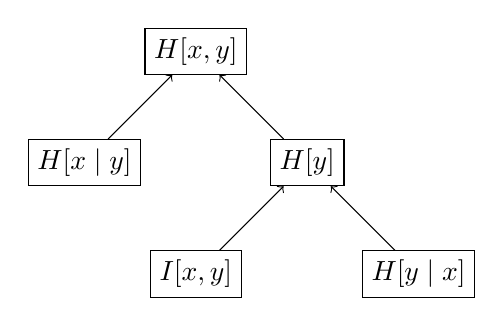
\begin{tikzpicture}[node distance=2cm]
        \node (Hxy) [draw, rectangle] {$H[x,y]$};
        \node (Hx) [draw, rectangle, below left of=Hxy] {$H[x\mid y]$};
        \node (Hy) [draw, rectangle, below right of=Hxy] {$H[y]$};
        \node (Hxyx) [draw, rectangle, below right of=Hy] {$H[y\mid x]$};
        \node (Ixy) [draw, rectangle, below left of=Hy] {$I[x,y]$};

        \draw[->] (Ixy) -- (Hy);
        \draw[->] (Hx) -- (Hxy);
        \draw[->] (Hy) -- (Hxy);
        \draw[->] (Hxyx) -- (Hy);
   
        
    \end{tikzpicture}
\end{center}
remark: the arrow means the left quantity add the right quantity equals the top quantity.

\section*{1.41}
Using the sum and product rules of probability, show that the mutual
information $I[x,y]$ satisfies the relation (1.121).
\begin{align*}
 I[x,y]&=-\int\int p(x,y)\ln(\frac{p(x)p(y)}{p(x,y)})dxdy=-\int \ln (p(x))dx\int p(x,y)dy+\int\int p(x,y)\ln(\frac{p(x,y)}{p(y)})dxdy \\
 &=-\int p(x)\ln(p(x))dx+\int\int p(x,y)\ln(p(x\mid y))dxdy=H[x]-H[x\mid y]   
\end{align*}

similarly, we can show that $I[x,y]=H[y]-H[y\mid x]$.
\section*{2.6}
Make use of the result (2.265) to show that the mean, variance, and mode of
the beta distribution (2.13) are given respectively by
\begin{align}
    \mathbb{E}[\mu] &= \frac{a}{a+b} \tag{2.267}\\
    \operatorname{var}[\mu] &= \frac{ab}{(a+b)^2(a+b+1)} \tag{2.268}\\
    \operatorname{mode}[\mu] &= \frac{a-1}{a+b-2}. \tag{2.269}
\end{align}

\[
E[\mu]=\int_{0}^{1}Beta(\mu \mid a,b)\mu d\mu=\frac{\Gamma(a+b)}{\Gamma(a)\Gamma(b)}\int_{0}^{1}\mu^{a}(1-\mu)^{b-1}d\mu=\frac{\Gamma(a+b)\Gamma(a+1)}{\Gamma(a)\Gamma(a+b+1)}=\frac{a}{a+b}
\]
\begin{align*}
    var[\mu]&=E[\mu^2]-E[\mu]^2=\int_{0}^{1}Beta(\mu \mid a,b)\mu^2 d\mu-(\frac{a}{a+b})^2\\
    &=\frac{\Gamma(a+b)}{\Gamma(a)\Gamma(b)}\int_{0}^{1}\mu^{a+1}(1-\mu)^{b-1}d\mu-(\frac{a}{a+b})^2\\
    &=\frac{\Gamma(a+b)\Gamma(a+2)}{\Gamma(a)\Gamma(a+b+2)}-(\frac{a}{a+b})^2\\
    &=\frac{ab}{(a+b)^2(a+b+1)}
\end{align*}

\[
\frac{d Beta(\mu \mid a,b)}{d \mu}=\frac{\Gamma(a+b)}{\Gamma(a)\Gamma(b)}((a-1)\mu^{a-2}(1-\mu)^{b-1}-(b-1)\mu^{a-1}(1-\mu)^{b-2})=0
\]
So, 
\[
mode[\mu]=\frac{a-1}{a+b-2}
\]


\section*{2.13}
Evaluate the Kullback--Leibler divergence (1.113) between two Gaussians
$p(\bm{x})=\mathcal{N}(\bm{x}\mid\bm{\mu},\bm{\Sigma})$ and
$q(\bm{x})=\mathcal{N}(\bm{x}\mid\bm{m},\bm{L})$.

\[
KL(p\mid \mid q)=-\int p(x)ln(q(x))dx+\int p(xln(p(x)))dx=-\int p(x)ln{\frac{q(x)}{p(x)}}dx
\]
\[
p(x)=N(x \mid \mu , \Sigma)=\frac{1}{(2\pi)^{D/2}\lvert\Sigma\rvert^{1/2}}exp(-\frac{1}{2}(x-\mu)^T\Sigma^{-1}(x-\mu))
\]
\[
q(x)=N(x \mid m,L)=\frac{1}{(2\pi)^{D/2}\lvert L\rvert^{1/2}}exp(-\frac{1}{2}(x-m)^TL^{-1}(x-m))
\]
So,
\[
KL(p\mid\mid q)=-\int \frac{1}{(2\pi)^{D/2}\lvert\Sigma\rvert^{1/2}} e^{-\frac{1}{2}(x-\mu)^T\Sigma^{-1}(x-\mu)} \ln \frac{|\Sigma|^{1/2}}{|L|^{1/2}}e^{\frac{1}{2}(x-\mu)^T\Sigma^{-1}(x-\mu)-\frac{1}{2}(x-m)^TL^{-1}(x-m)}dx
\]
\[
\mathrm{KL}(p\|q)
=\frac12\log\frac{|L|}{|\Sigma|}
-\frac12\mathbb E_p[(x-\mu)^T\Sigma^{-1}(x-\mu)]
+\frac12\mathbb E_p[(x-m)^TL^{-1}(x-m)].
\]
let $z=x-\mu$, we have $z\sim N(0,\Sigma)$, so
\[
\mathbb E[z^T\Sigma^{-1}z]
=\operatorname{tr}(\Sigma^{-1}\Sigma)=D.
\]
similarly,
\begin{align*}
\mathbb E[(z+\mu - m)^T L^{-1} (z+\mu -m)]&=\mathbb E \operatorname{tr}((z+\mu - m)^T L^{-1} (z+\mu -m))=\mathbb E \operatorname{tr}{L^{-1} (z+\mu -m)(z+\mu - m)^T} \\
&=\operatorname{tr}(L^{-1}\Sigma)+(\mu-m)^TL^{-1}(\mu-m)=tr(L^{-1}\Sigma)+(\mu-m)^TL^{-1}(\mu-m)
\end{align*}
\[ 
\mathrm{KL}(p\|q)
=\frac12\left[
\log\frac{|L|}{|\Sigma|}
-D+\operatorname{tr}(L^{-1}\Sigma)
+(\mu-m)^TL^{-1}(\mu-m)
\right].
\]
\section*{2.15}
Show that the entropy of the multivariate Gaussian
$\mathcal{N}(\bm{x}\mid\bm{\mu},\bm{\Sigma})$ is given by
\begin{equation}
    H[\bm{x}] = \frac{1}{2}\ln\lvert\bm{\Sigma}\rvert
    + \frac{D}{2}\bigl(1+\ln(2\pi)\bigr)
    \tag{2.283}
\end{equation}
where $D$ is the dimensionality of $\bm{x}$.

\[
\int p(x)(x-\mu)^T\Sigma^{-1}(x-\mu)dx=\mathbb E((x-\mu)^T\Sigma^{-1}(x-\mu))=\operatorname{tr}(\Sigma^{-1}\Sigma)=D.
\]
\begin{align*}
    H[x]&=-\int p(x) \ln (p(x))dx=-\int \frac{1}{(2\pi)^{D/2}\lvert\Sigma\rvert^{1/2}} e^{-\frac{1}{2}(x-\mu)^T\Sigma^{-1}(x-\mu)} \ln \frac{1}{(2\pi)^{D/2}\lvert\Sigma\rvert^{1/2}} e^{-\frac{1}{2}(x-\mu)^T\Sigma^{-1}(x-\mu)} dx\\
    &=\frac{1}{2}\ln \lvert \Sigma \rvert + \frac{D}{2}\ln(2\pi)+\frac{1}{2}\int p(x)(x-\mu)^T\Sigma^{-1}(x-\mu)dx\\
    &=\frac{1}{2}\ln \lvert \Sigma \rvert + \frac{D}{2}\ln(2\pi)+\frac{D}{2}
\end{align*}
\section*{2.26}
A very useful result from linear algebra is the \emph{Woodbury} matrix
inversion formula given by
\begin{equation}
    (\bm{A}+\bm{B}\bm{C}\bm{D})^{-1}
    = \bm{A}^{-1} - \bm{A}^{-1}\bm{B}
    (\bm{C}^{-1}+\bm{D}\bm{A}^{-1}\bm{B})^{-1}
    \bm{D}\bm{A}^{-1}.
    \tag{2.289}
\end{equation}
By multiplying both sides by $(\bm{A}+\bm{B}\bm{C}\bm{D})$ prove the
correctness of this result.

Left multiltiplying both side by $(\bm{A}+\bm{B}\bm{C}\bm{D})$ gives
\[
LHS=I_n
\]
\[
RHS=I_n-B(C^{-1}+DA^{-1}B)^{-1}DA^{-1}+BCDA^{-1}-BCDA^{-1}b(C^{-1}+DA^{-1}B)^{-1}DA^{-1}
\]
next prove  $-B(C^{-1}+DA^{-1}B)^{-1}DA^{-1}+BCDA^{-1}-BCDA^{-1}B(C^{-1}+DA^{-1}B)^{-1}DA^{-1}=O$
i.e.$-(C^{-1}+DA^{-1}B)^{-1}D+CD-CDA^{-1}B(C^{-1}+DA^{-1}B)^{-1}D=O$

i.e.
\[
C(C^{-1}+D(A^{-1}B))-CDA^{-1}B=I_n
\]
Obviously, this is true. we have $LHS=RHS$.
Since, the matrix space is a commutative ring, we can also prove the right multiplication by $(\bm{A}+\bm{B}\bm{C}\bm{D})$ gives the same result.
\section*{2.29}
Using the partitioned matrix inversion formula (2.76), show that the
inverse of the precision matrix (2.104) is given by the covariance
matrix (2.105).

\[
R=
\begin{pmatrix}I&-A^T\\0&I\end{pmatrix}
\begin{pmatrix}\Lambda&0\\0&L\end{pmatrix}
\begin{pmatrix}I&0\\-A&I\end{pmatrix}.
\]
So,
\[
R^{-1}=\begin{pmatrix}I&0\\-A&I\end{pmatrix}^{-1}\begin{pmatrix}\Lambda&0\\0&L\end{pmatrix}^{-1}\begin{pmatrix}I&-A^T\\0&I\end{pmatrix}^{-1}
\]
By (2.76), we have
\[
\begin{pmatrix}I&0\\-A&I\end{pmatrix}^{-1}=\begin{pmatrix}
I&0\\A&I
\end{pmatrix}
\]
\[
\begin{pmatrix}\Lambda&0\\0&L\end{pmatrix}^{-1}=\begin{pmatrix}
\Lambda^{-1}&0\\0&L^{-1}
\end{pmatrix}
\]
\[
\begin{pmatrix}I&-A^T\\0&I\end{pmatrix}^{-1}=\begin{pmatrix}
I&A^T\\0&I
\end{pmatrix}
\]
So,
\[
R^{-1}=\begin{pmatrix}
    \Lambda^{-1}&\Lambda^{-1}A^T\\
    A\Lambda^{-1}&L^{-1}+A\Lambda^{-1}A^T
\end{pmatrix}
\]
\end{document}


